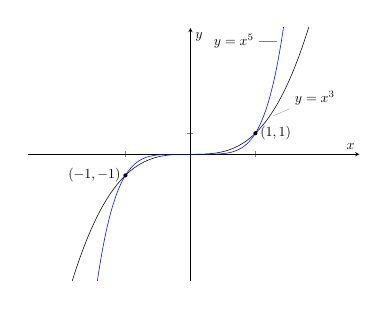
\begin{tikzpicture}[scale=0.5]
\begin{axis}[
%title = {$f(x)=x^n$, $n=2k+1$, $k \in \mathrm{Z}_{+}$},
 axis lines=middle,
 ticklabel style={fill=white},
 xmin=-2.5,xmax=2.6,
 ymin=-6,ymax=6,
 xlabel=$x$,ylabel=$y$,
 domain=-2:2,
 samples=100,
 smooth,
 xtick={-1,0,1},ytick={1},
 yticklabels={,,},   xticklabels={,,},
 width=10cm, height=8cm]
\coordinate  (x2) at (1,1);
\coordinate (x1) at (-1,-1);

\addplot[black] { x^3};
\addplot[blue] {x^5};

\fill[black] (x1) circle (1.5pt);
\fill[black] (x2) circle (1.5pt);

\node[pin= 20:{$y=x^3$}] at (axis cs:1.2,{(1.2)^3}) {};
\node[pin= 180:{$y=x^5$}] at (axis cs:1.4,{(1.4)^5}) {};

\node[right] at (x2) {$(1,1)$};
\node[left] at (x1) {$(-1,-1)$};
\end{axis}
\end{tikzpicture}